%!TEX root = ../main.tex
\section{Advantages} % (fold)
\label{sec:advantages}

\subsection{Capturing a sinusoidal flow} % (fold)
\label{sub:capturing_a_sinusoidal_flow}

Harmonic balance approaches have been developed to
efficiently capture unsteady periodic signals.
In order to set these ideas on a simple example,
let us take the case of an injected signal composed
of the sum of two sine functions: 
\begin{equation}
	u_0(t) = \sin (2 \pi f_1 t) + \sin(2 \pi f_2 t).
\end{equation}




\subsubsection{case 1: $f_1 = f_2 = 1 \text{Hz}$}

This signal is made of a single frequency $f_1 = f_2 = 1 \text{Hz}$.
The mono-frequential harmonic balance computation ran with only one harmonic
is shown Fig.~\ref{fig:convection_sin_1_tsm_n_1}.
\begin{figure}[htbp]
  \begin{center}
    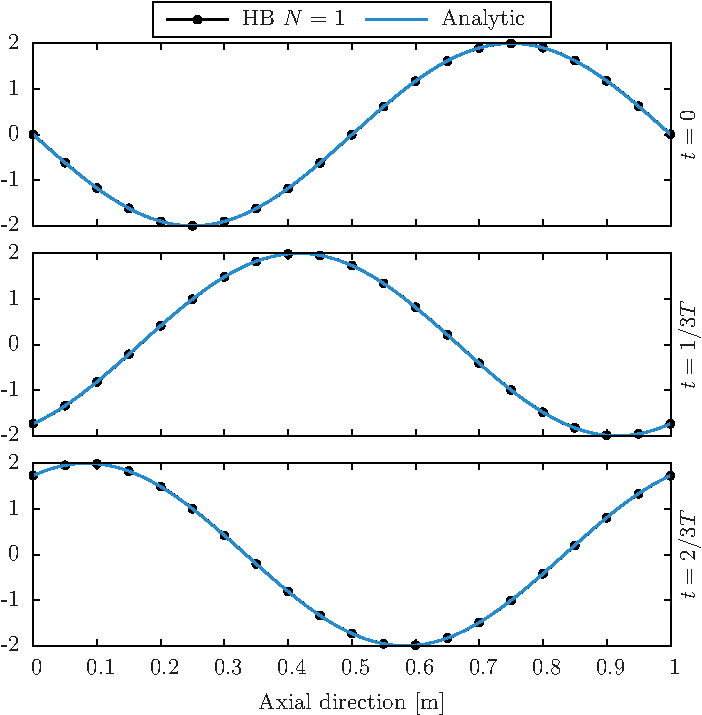
\includegraphics[width=.5\textwidth]{CONVECTION/FIGS/CONVECTION_SIN_1_TSM_N1.pdf}
  \end{center}
  \caption{Convection of a sinusoidal function. Harmonic balance computation
  ran with $f_1$ frequency compared to analytical result}
  \label{fig:convection_sin_1_tsm_n_1}
\end{figure}
The harmonic balance results match perfectly the analytical solution.
This was expected as harmonic balance methods have been developed to
easily capture periodic signals. When these are made of only one frequency,
one harmonic is sufficient to capture all the unsteadiness.

\subsubsection{$f_1 = 1 \text{Hz}$, $f_2 = 2 \text{Hz}$}

A sinusoidal function with a frequency $f_2 = 2f_1$ is now injected.
Two computations are ran. The first has 

\begin{figure}[htbp]
  \begin{center}
    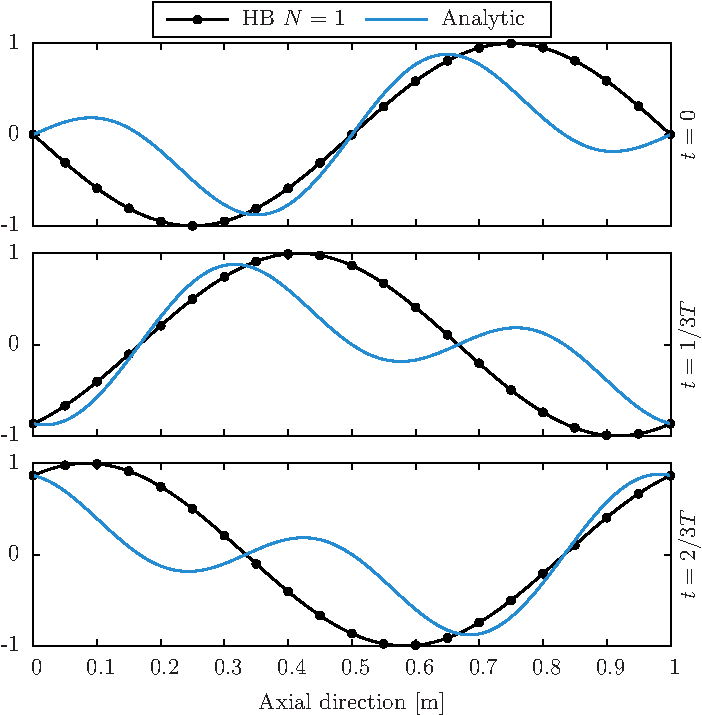
\includegraphics[width=.5\textwidth]{CONVECTION/FIGS/CONVECTION_SIN_2_TSM_N1.pdf}
  \end{center}
  \caption{Convection of a sinusoidal function. Harmonic balance computation
  ran with frequency compared to analytical result}
  \label{fig:convection_sin_2_tsm_n_1}
\end{figure}

\begin{figure}[htbp]
  \begin{center}
    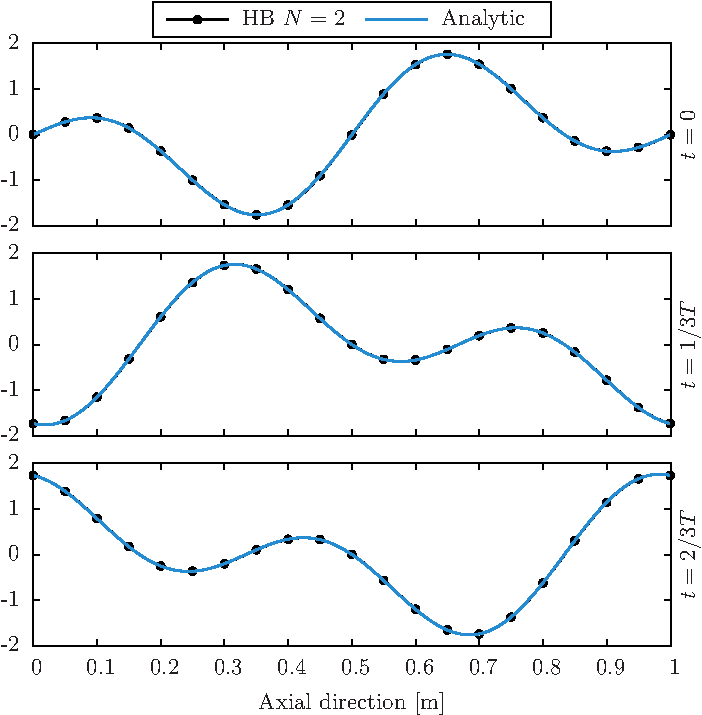
\includegraphics[width=.5\textwidth]{CONVECTION/FIGS/CONVECTION_SIN_2_TSM_N2.pdf}
  \end{center}
  \caption{Convection of a sinusoidal function.}
  \label{fig:convection_sin_2_tsm_n_2}
\end{figure}

\subsubsection{$f_1 = 1 \text{Hz}$, $f_2 = 10 \text{Hz}$}




\underline{What we have learned:} 
\begin{itemize}
  \item from case 1: For a sinusoidal temporal function made of only one frequency,
        only one frequency is needed to capture the field. This is much more efficient
        than a classical time-marching scheme.
\end{itemize}



% subsection capturing_a_sinusoidal_flow (end)

% section advantages (end)